
%--------------------------------------------------------------------
%--------------------------------------------------------------------
% Formato para los talleres del curso de Herramientas Computacionales
% Universidad de los Andes
% 2015-10
%--------------------------------------------------------------------
%--------------------------------------------------------------------

\documentclass[11pt,letterpaper]{exam}
\usepackage[utf8]{inputenc}
\usepackage[spanish]{babel}
\usepackage{graphicx}
\usepackage{mdframed}
\usepackage{tabularx}
\usepackage[absolute]{textpos} % Para poner una imagen completa en la portada
\usepackage{multirow}
\mdfdefinestyle{mystyle}{leftmargin=1cm,rightmargin=1cm,linecolor=red}
\usepackage{float}
\usepackage{hyperref}
\usepackage{listings}
\lstset{
basicstyle=\ttfamily,
keepspaces=true,
columns=flexible
}
\decimalpoint
%\usepackage{pst-barcode}
%\usepackage{auto-pst-pdf}

\newcommand{\base}[1]{\underline{\hspace{#1}}}
\boxedpoints
\pointname{ pt}
%\extrawidth{0.75in}
%\extrafootheight{-0.5in}
\extraheadheight{-0.15in}
%\pagestyle{head}

%\noprintanswers
%\printanswers
\renewcommand{\solutiontitle}{}
\SolutionEmphasis{\color{blue}}

\usepackage{upquote,textcomp}
\newcommand\upquote[1]{\textquotesingle#1\textquotesingle} % To fix straight quotes in verbatim

\begin{document}
\begin{center}
{\Large Herramientas Computacionales} \\
Taller 4 - \textsc{Python}:\\
Operaciones aritméticas, listas, condicionales \\
 cadenas de caracteres y estructuras iterativas. \\
Fecha de publicación: {\small \it febrero 25 de 2015}\\
\end{center}

\begin{textblock*}{40mm}(10mm,20mm)
  
\includegraphics[width=3cm]{logoUniandes.png}
\end{textblock*}

\begin{textblock*}{40mm}(161mm,20mm)
  
\includegraphics[width=3cm]{logoUniandes.png}
\end{textblock*}

\vspace{0.5cm}

Los programas que resuelven este taller deben ser entregados en un solo archivo con nombre \verb+NombreApellido_HW4.zip+ o como parte de un cuaderno de iPython con nombre \verb+NombreApellido_HW4.ipynb+.

En cada ejercicio se entrega 1/3  de los puntos si el código propuesto es razonable, 1/3 si se puede ejecutar y 1/3 si entrega resultados correctos. 

{\bf Las respuestas deben llevar comentarios suficientes que expliquen la solución propuesta.}


\vspace{0.5cm}


\begin{questions}

\question[50] {\bf Imprimiendo en espiral}
Escriba un programa que guarde en una lista de listas en espiral y en el sentido de las manecillas del reloj los números del $1$ a $49$. El programa debe imprimir los números en pantalla, separados por un espacio. Llámelo \verb+espiral.py+.

\begin{center}
	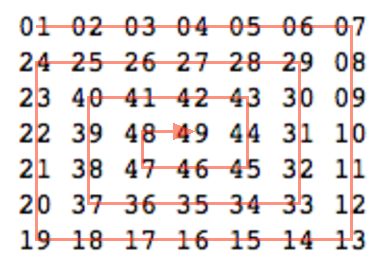
\includegraphics[width=0.2\textwidth]{./spiral7.pdf}
\end{center}

%\part[20] Escriba un programa que haga lo mismo en el sentido en contra de las manecillas del reloj para una matriz cuadrada de $8\times8$. Llámelo \verb+contraespiral_reloj.py+.
%
%\begin{center}
%	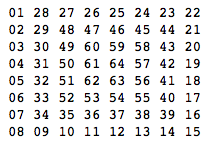
\includegraphics[width=0.23\textwidth]{./antispiral8.png}
%\end{center}
%
%\end{parts}

\question[50] {\bf Criptografía}
Un mensaje se ha codificado en dos etapas. Primero se ha tomado cada caracter y a su código ASCII se le ha sumado $(n\%5)$ siendo $n$ la posición del caracter en el mensaje (comenzando en $1$). Después se ha invertido el orden de los caracteres. El mensaje codificado se muestra a continuación, todo siendo \textbf{una sola línea}. Escriba un programa en Python llamado \verb+uncripto.py+ que descifre el mensaje.

\begin{center}
	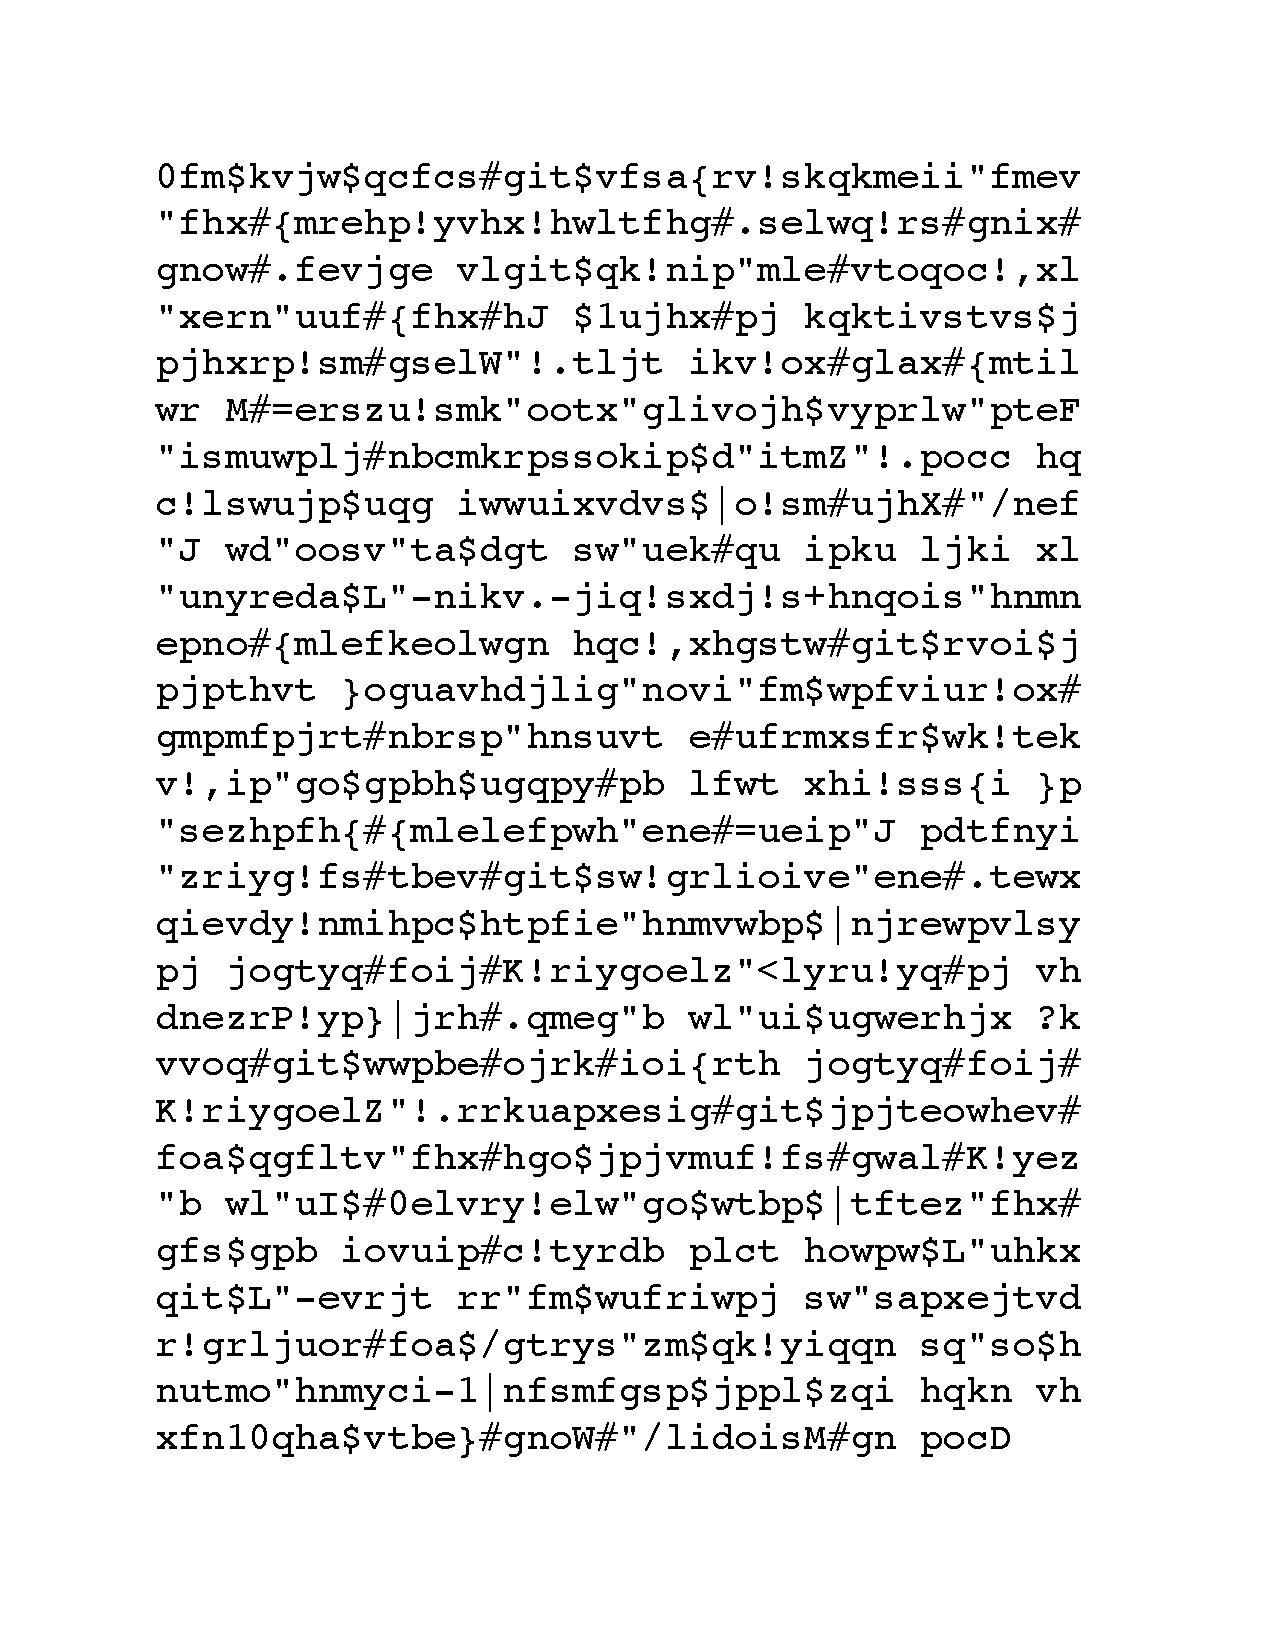
\includegraphics[width=0.40\textwidth]{./encrypted.pdf}
\end{center}

%\newpage
%
%\begin{center}
%	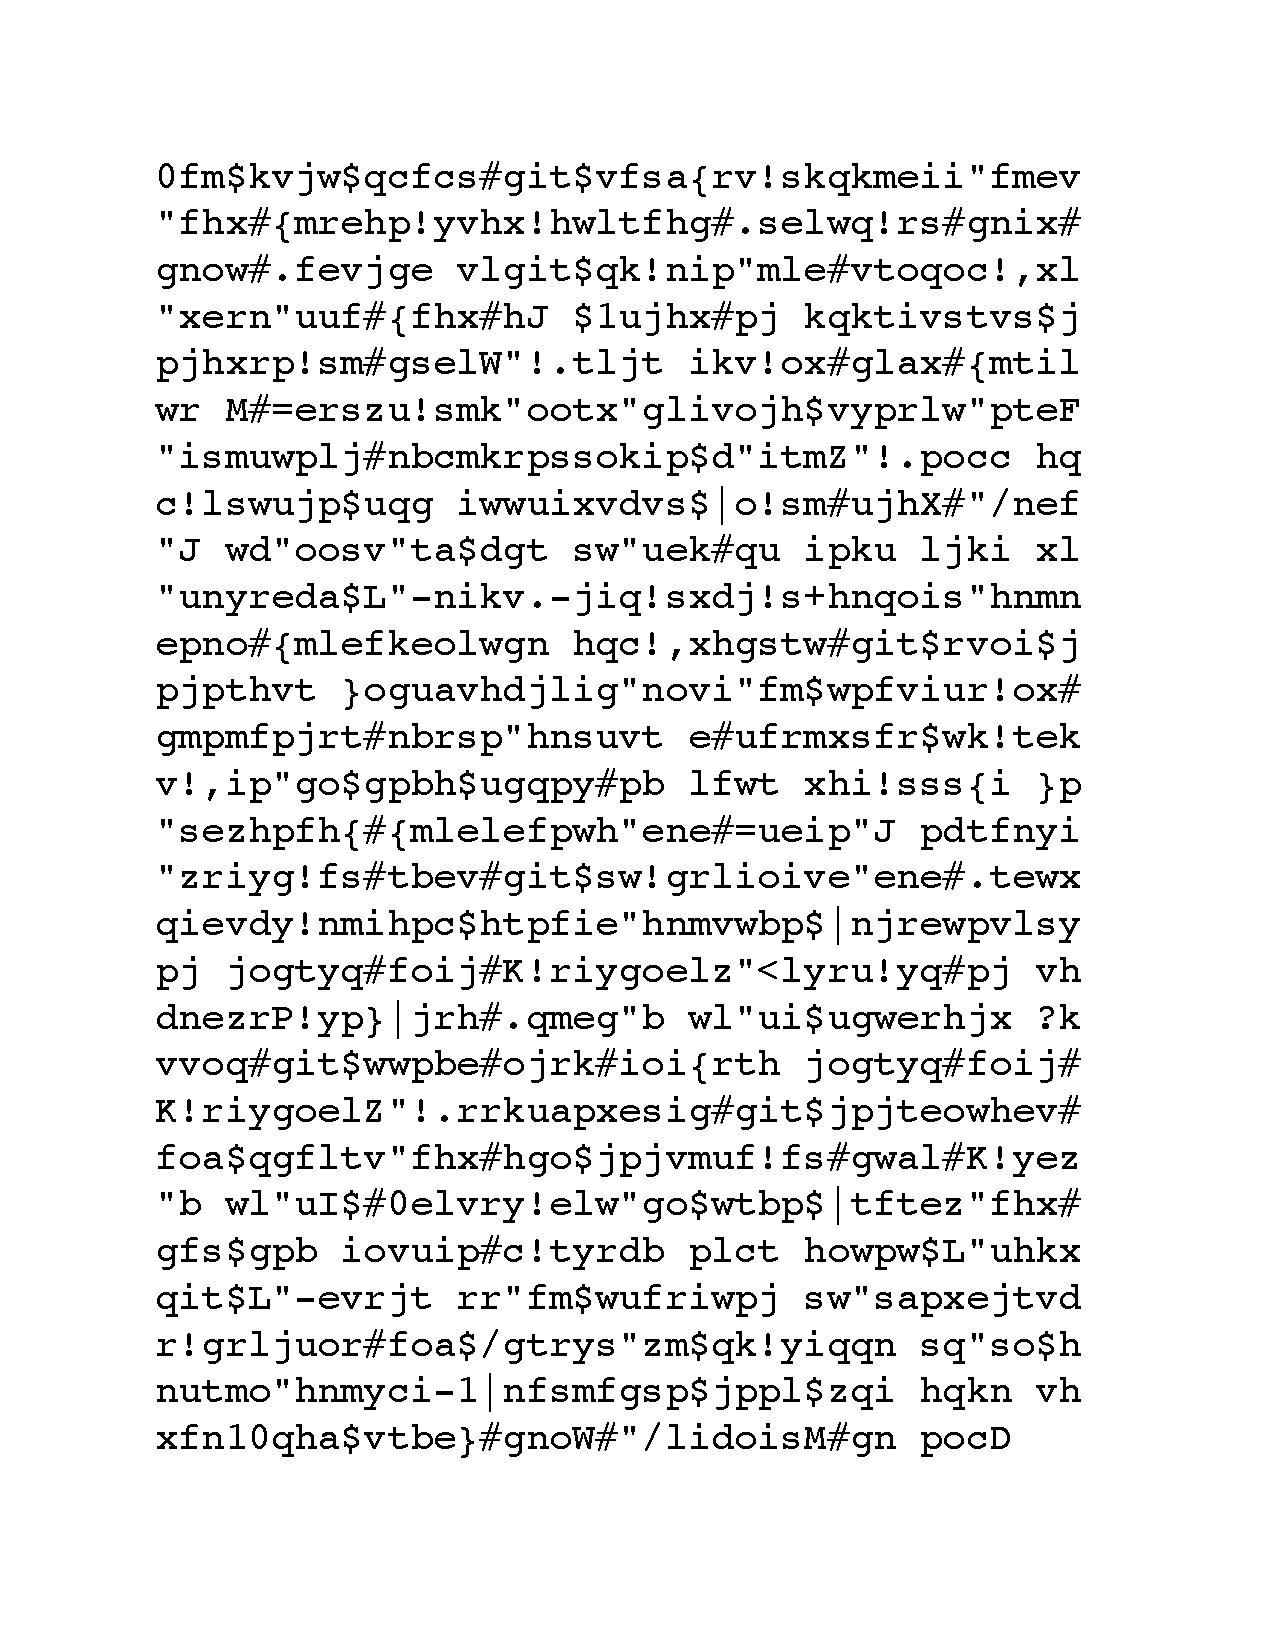
\includegraphics[width=0.95\textwidth]{./encrypted.pdf}
%\end{center}

\end{questions}


\end{document}
